\section{Fourier Methods and Spectrograms}
\label{sec:fourier_methods_and_spectrograms}

Spectrograms have a long history but were first used with machine learning models to synthesise music at the start of the 21st century\cite{NoteOnsetDetection}.

The time-domain based audio signal was divided into equal lengths of shorter periods. Then, a Fast Fourier Transform (FFT) is applied to each segment, decomposing the signal at each of the timestep periods into its constituent frequencies and corresponding amplitude. The complex values from the Fast Fourier Transform are complex values, giving spectrograms of frequency and phase.

A spectrogram is a graphical plot of the decomposition of sound using the \acrfull{STFT}. It consists of 2 plots frequency against time and phase against time. Each point of the plots is coloured in amplitude/intensity of the decomposed audio signal at a specific point in time. The STFT is a sum of overlapped Fast Fourier Transforms (FFTs) of the audio signal. After calculation of the STFT, the sample is divided into overlapping frames of equal length, known as the hamming window. Finally, the FFT is then applied to each audio signal frame. The outputted complex functions from the Fast Fourier Transform give spectrograms of amplitude and phase of different frequencies at each timestep.

\subsection{Mel-Spectrograms}

Mel Spectrograms are an adaptation of the spectrograms more suited to sounds intended to be heard by humans. Mel Spectrograms have amplitude/sound intensity adjusted along a logarithmic scale such that graphical distances between frequencies sound the same distance as human hearing would detect them to be. This adjustment enables machine learning models to learn how to produce audio sequences that sound more natural to a human listener.

\begin{figure}[H]
    \centering
    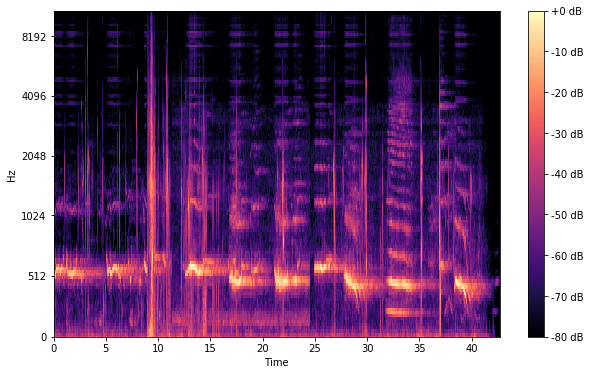
\includegraphics[width=0.8\textwidth]{literature_review/MelSpectrogram.png}
    \caption{An example of a  Mel Spectrogram showing the amplitude of different frequencies in a sound over time\cite{GettingToKnowTheMelSpectrogram}}
    \label{fig:spectrograms}
\end{figure}

There is no standardised formula for converting frequncy onto the mel logarhthmic scale as it is up to interpretation the adjustment level that is required for human hearing, though then most common formula is\cite{SpeechCommunication}:

\begin{equation}
    m = 2596 log(1 +  \frac{f}{700}) = 1127 ln (1 + \frac{f}{700})
\end{equation}

\subsection{Intepreting Phase}

The STFT is a complex function; however, only the magnitude part is currently utilised by most models, and the phase part is discarded. Any reconstructed signal cannot have the same phase as the original signal if the phase information is lost. Human hearing is capable of distinguishing between two sounds with the same frequency, but with different phases, meaning that sounds resynthesized without phase can sound unnatural and different to the original, regardless of the frequency.

Success at interpreting the phase spectrogram to date has been limited. As a result, most models discard the phase part of the signal and make models purely off the frequency spectrogram. Discarding the phase is a problem as the phase is a crucial part of spectrogram representation, making the image representation fully convertible back to audio, though it is challenging to work with for several reasons:

Firstly, the phase spectrogram appears random, making it challenging to distinguish meaningful information from noise.

Secondly, the spectrogram phase is a cyclic quality. Cyclic qualities are more challenging to interpret than non-cyclic qualities as they are not continuous. One paper called GANSynth\cite{GANSynth} overcomes this problem by calculating the phase difference between individual timesteps of a spectrogram and making $2\pi$  adjustments for when the phase wraps around. This phase difference is called the instantaneous frequency and provides far more informative information than the raw phase. Instantaneous frequency over harmonics, for instance, is expected to be constant.

\begin{figure}[H]
    \centering
    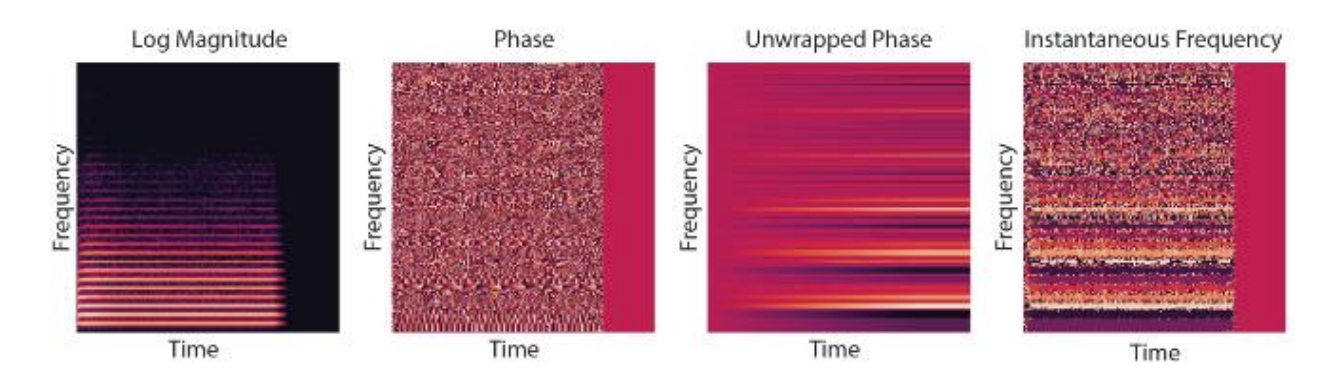
\includegraphics[width=0.8\textwidth]{literature_review/PhaseAdjustment.png}
    \caption{UnwrappingSpectrogram Phase: An illustration from the GANSynth paper of how the phase of a spectrogram is adjusted to make it more interpretable to a neural network\cite{GANSynth}}
    \label{fig:phase_unwrapping}
\end{figure}

\subsection{Spectrogram Evaluation}

Spectrogram based encoding for music sound synthesis is currently the best method for encoding musical sounds due to their ease of use and the low-level control over signal information that does not hinder their interpretation (unlike raw waveform encoding). Conventional image processing models, e.g. Convolutional Neural Networks or Recurrent Neural Networks, can be used to process the spectrogram. These models can extract local sounds at specific frequencies from a spectrogram and learn how to reproduce them. This extraction is possible due to the separated frequency and timewise position of sounds that form specific image patterns that an autoencoder can be trained to recognise. An example in this case of singing is shown in the following Figure \ref{fig:spectrogram_features}:

\begin{figure}[H]
    \centering
    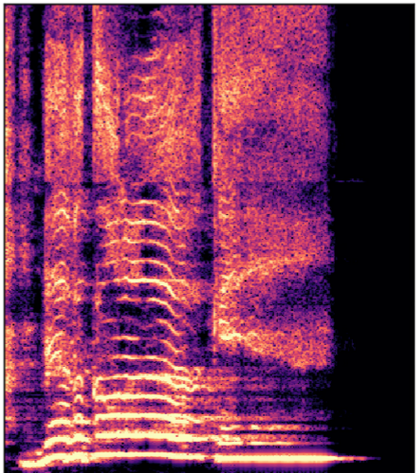
\includegraphics[width=0.4\textwidth]{literature_review/SpectrogramFeatures.png}
    \caption{Spectrogram Features: Regular harmonics present in singing can be observed in the bright horizontal regions of the spectrogram that repeat at regular frequency intervals. A model could be trained to extract these features and learn to resynthesize them}
    \label{fig:spectrogram_features}
\end{figure}


Additionally, one of their defining advantages is that they can be used to reconstruct the original audio signal from the spectrogram with the inverse Fourier Transform. The reconstructed audio signal will be almost identical to the original (phase-matched) if phase and magnitude spectrograms are used.
Spectrograms are at the core of many recently published music synthesis models and papers, showing academic relevance.

However, most models based on spectrograms, e.g. raw CNN-based models, are limited and do not make use of biases in sound, for instance, the tendency of natural sounds to oscillate sinusoidally at harmonic frequencies according to the harmonic plus noise model. In addition, many traditional autoencoder-based RNN models do not enable the configuration of specific sound features, e.g. fundamental frequency or loudness. Additionally, spectrogram based models are not without problems (e.g. the discarding phase of information).

Therefore spectrograms, although helpful, cannot be used to synthesise audio signals on their own; to achieve widespread academic and commercial use, a different representation to help a model relate them to sound is required, for example, \nameref{section:DDSP}.